% A Readymade beamer presentation template
% Version 1.1
% Relase date: May 2, 2010
% Released at http://www.stattler.com
% by Rifat Jahan

\documentclass[12pt]{beamer}
%\usecolortheme[named=green]{structure}
\mode<presentation> {
\usetheme{Madrid} % My favorite!
%\usetheme{Boadilla} % Pretty neat, soft color.
%\usetheme{default}
%\usetheme{Warsaw}
%\usetheme{Bergen} % This template has nagivation on the left
%\usetheme{Frankfurt} % Similar to the default with an extra region at the top.
%\usecolortheme{seahorse} % Simple and clean template
%\usetheme{Darmstadt} % not so good
% Uncomment the following line if you want page numbers and using Warsaw theme
% \setbeamertemplate{footline}[page number]
%\setbeamercovered{transparent}
\setbeamercovered{invisible}
% To remove the navigation symbols from the bottom of slides%
\setbeamertemplate{navigation symbols}{}
}

\usepackage{graphicx}
%\logo{
\includegraphics[height=0.6cm]{../../openbr.png}}
\title[OpenBR]{OpenBR -- Open Source Biometric Recognition}
\author[J. Klontz \& B. Klare \& M. Burge]{Josh Klontz \& Brendan Klare \& Mark Burge}
\institute[]
{
www.openbiometrics.org \\
\medskip
{\emph{openbr-dev@googlegroups.com}}
}
\date{\today}

\begin{document}

\begin{frame}
\titlepage
\end{frame}

\section{Introduction}
\begin{frame}
\frametitle{Motivation}
\begin{block}
{Why Open Source?}
Brendan's passionate speech on the need for open source biometrics software!
\end{block}
\end{frame}

\begin{frame}
\frametitle{What's in it?}
\begin{itemize}
\item Off-the-shelf algorithms
  \begin{itemize}
  \item Face Recognition
  \item Gender Classification
  \item Age Estimation
  \item Commercial Wrappers
  \end{itemize}
\pause
\item Tools for algorithm evaluation
  \begin{itemize}
  \item Standardized set of file formats
  \item Automatic plot generation
  \item Command line interface supporting common use cases
  \end{itemize}
\pause
\item Software framework for algorithm development
  \begin{itemize}
  \item C++ plugin API for implementing new algorithms
  \item Grammar for image processing
  \item Automatic packaging and deployment
  \item Source code hosted on GitHub!
  \end{itemize}
\end{itemize}
\end{frame}

\newcommand{\graphicblock}[3]
{
  \begin{block}{#1}
    \begin{columns}
      \column{0.1\textwidth}
        \includegraphics[width=\textwidth]{#2}
      \column{0.9\textwidth}
        #3
    \end{columns}
  \end{block}
}

\begin{frame}[fragile]
\frametitle{Software Architecture}
\begin{columns}
\column{.48\textwidth}
  \graphicblock{Qt}{img/qt}{Cross-platform application and UI framework}
  \graphicblock{OpenCV}{img/opencv}{Image processing library}
  \graphicblock{Eigen}{img/eigen}{Linear algebra library}
  \graphicblock{CMake}{img/cmake}{Cross-platform build system}
\pause
\column{.48\textwidth}
  \graphicblock{br}{img/openbr}{Command line application for running algorithms and evaluating results.}
  \graphicblock{C API}{img/openbr}{High-level interface for other programming languages.}
  \graphicblock{C++ Plugin API}{img/openbr}{Core interface for using and developing algorithms.}
\end{columns}
\end{frame}

\begin{frame}
\frametitle{Supported Platforms}
\begin{columns}
\column{.3\textwidth}
  \begin{block}{Now}
  \centering
  
\includegraphics[height=0.2\textheight]{img/windows} \\
  
\includegraphics[height=0.2\textheight]{img/mac} \\
  
\includegraphics[height=0.2\textheight]{img/linux}
  \end{block}
\pause
\column{.3\textwidth}
  \begin{block}{Soon}
  \centering
  
\includegraphics[height=0.15\textheight]{img/android} \\
  
\includegraphics[height=0.15\textheight]{img/ios} \\
  
\includegraphics[height=0.15\textheight]{img/rpi} \\
  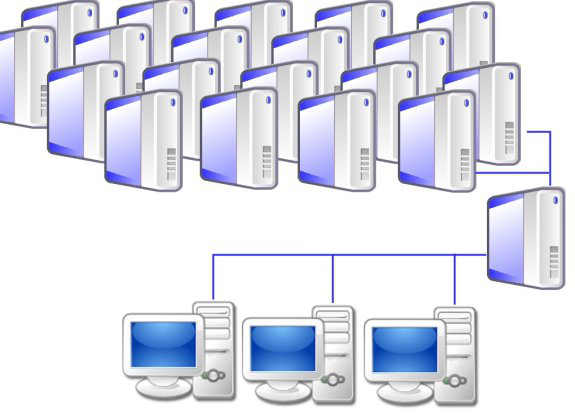
\includegraphics[height=0.15\textheight]{img/mpi}
  \end{block}
\pause
\column{.3\textwidth}
  \begin{block}{Future}
  \centering
  
\includegraphics[height=0.2\textheight]{img/phi} \\
  
\includegraphics[height=0.2\textheight]{img/nvidia} \\
  
\includegraphics[height=0.2\textheight]{img/apu}
  \end{block}
\end{columns}
\end{frame}

\begin{frame}
\frametitle{Algorithm Evaluation}
\begin{columns}
  \column{0.33\textwidth}
    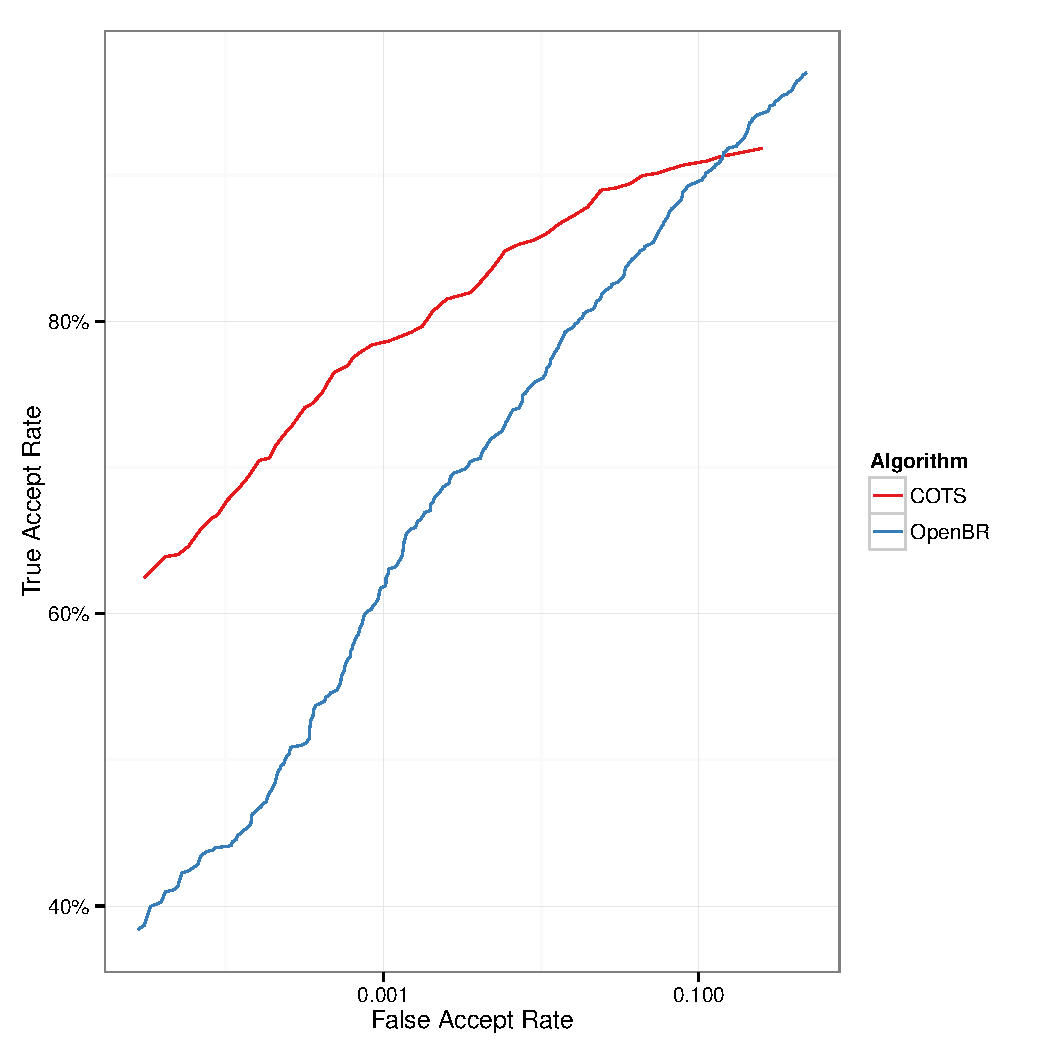
\includegraphics[width=\textwidth]{img/MEDS/MEDS_ROC}
  \column{0.33\textwidth}
    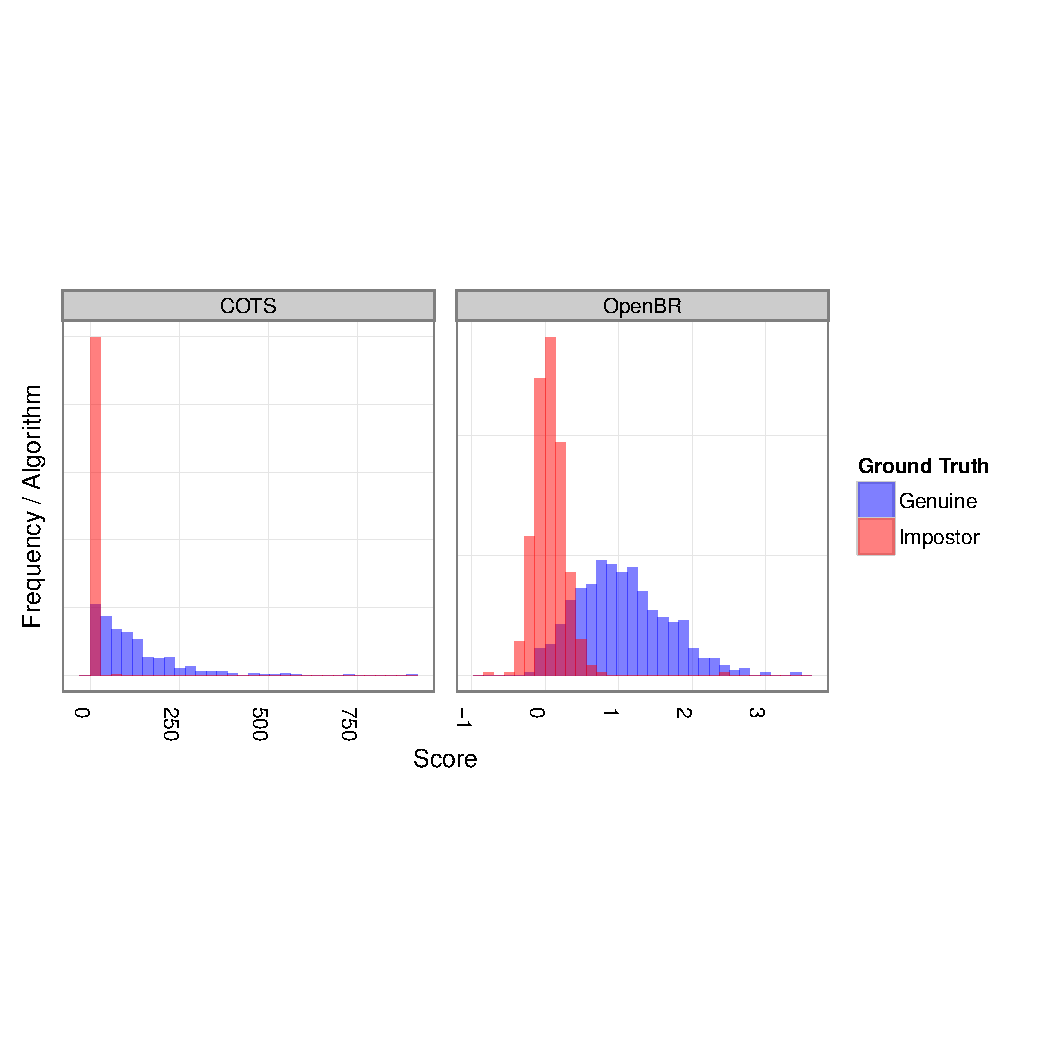
\includegraphics[width=\textwidth]{img/MEDS/MEDS_SD}
  \column{0.33\textwidth}
    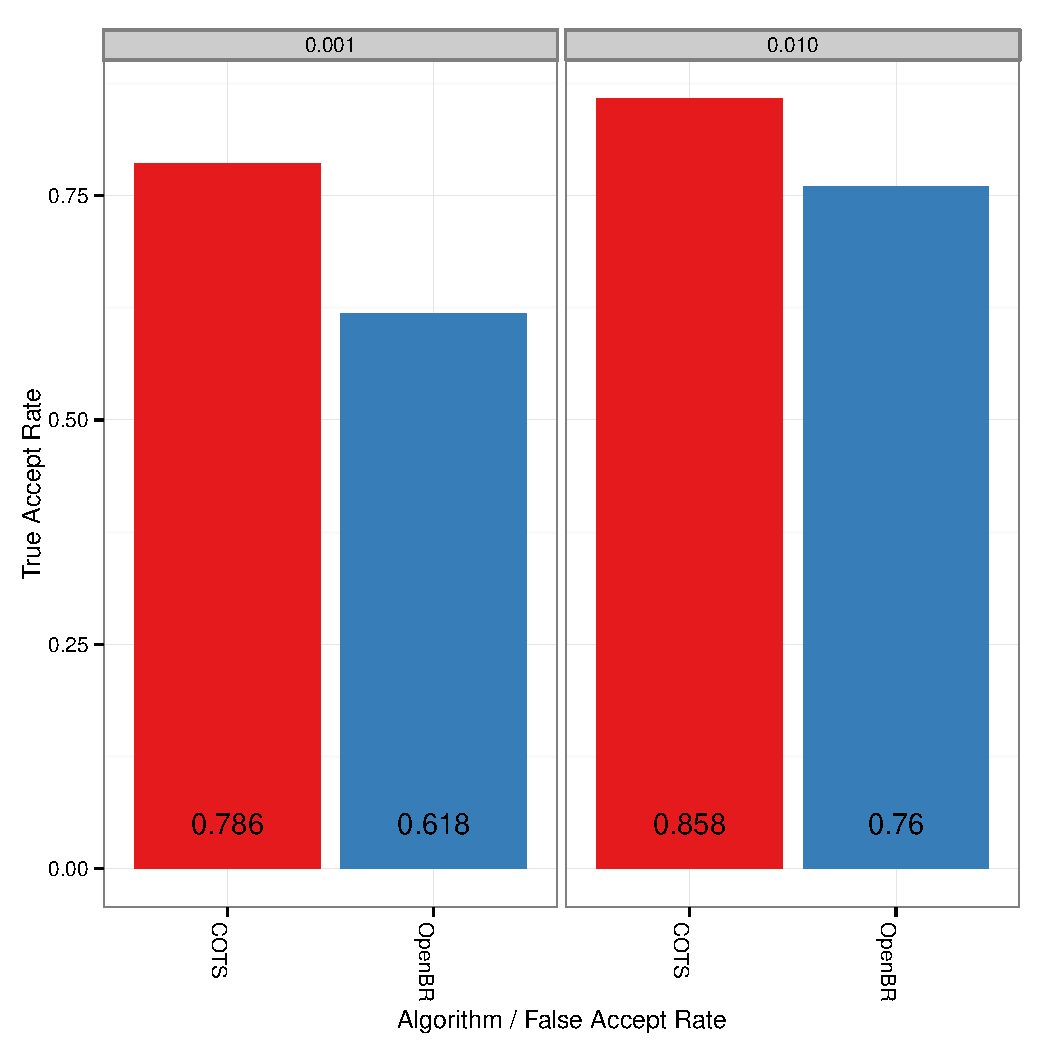
\includegraphics[width=\textwidth]{img/MEDS/MEDS_BC}
\end{columns}
\pause
\begin{block}{Requires \emph{R} Software Environment}
\textgreater \ install.packages(c("ggplot2", "gplots", "reshape", "scales"))
\end{block}
\pause
\begin{block}{}
\emph{ggplot2} is amazing!
\end{block}
\end{frame}

\begin{frame}[fragile]
\frametitle{Plugin Example: Local Binary Patterns}
{\footnotesize
\pause
\begin{verbatim}
#include <openbr_plugin.h>
\end{verbatim}
\vspace{-24pt}
\pause
\begin{verbatim}
class LBP : public Transform {
\end{verbatim}
\vspace{-24pt}
\pause
\begin{verbatim}
  BR_PROPERTY(int, radius, 1)
\end{verbatim}
\vspace{-24pt}
\pause
\begin{verbatim}
  void project(const Matrix &src, Matrix &dst) const {
\end{verbatim}
\vspace{-24pt}
\pause
\begin{verbatim}
    for (int r=radius; r<src.rows-radius; r++)
      for (int c=radius; c<src.cols-radius; c++) {
        float cval = p[(r+0*radius)*src.cols+c+0*radius];
        dst(r, c) =
          (p[(r-radius)*src.cols+c-radius] >= cval ? 128 : 0) |
          (p[(r-radius)*src.cols+c] >= cval ? 64 : 0) |
          ...;
      }
\end{verbatim}
\vspace{-24pt}
\pause
\begin{verbatim}
  }
};
\end{verbatim}
\vspace{-24pt}
\pause
\begin{verbatim}
BR_REGISTER(Transform, LBP)
\end{verbatim}
\vspace{-24pt}
\pause
\begin{verbatim}
...
Transform *lbp = Transform::make("LBP(3)");
\end{verbatim}
\vspace{-24pt}
\pause
\begin{verbatim}
Transform *lbpu2 = Transform::make("LBP(3)+U2");
\end{verbatim}
\vspace{-24pt}
\pause
\begin{verbatim}
Transform *fr = Transform::make("FaceDetection+FaceRegistration+
                                 LBP(3)+U2+RSLDA");
\end{verbatim}
}
\end{frame}

\begin{frame}
\frametitle{Welcome to the Parallel Jungle!}
\begin{figure}
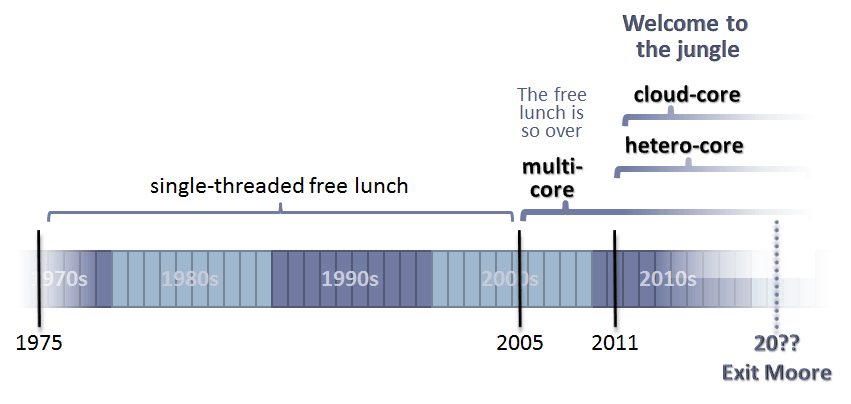
\includegraphics[width=\textwidth]{img/sutter.png}
\caption{http://www.drdobbs.com/parallel/welcome-to-the-parallel-jungle/232400273}
\end{figure}
\end{frame}

\begin{frame}
\frametitle{Economics}
\begin{columns}
\column{0.48\textwidth}
\begin{figure}
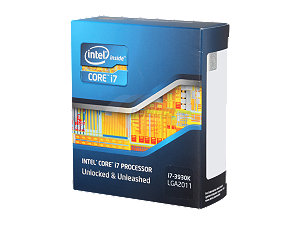
\includegraphics[width=.75\textwidth]{img/i73930k.png}
\caption{i7 3930k}
\end{figure}
\column{0.48\textwidth}
\begin{figure}
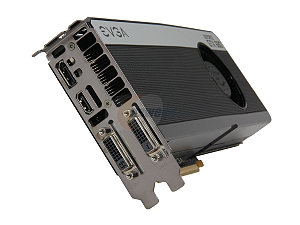
\includegraphics[width=.75\textwidth]{img/gtx680.png}
\caption{GTX 680}
\end{figure}
\end{columns}
\pause
\begin{columns}
\column{0.48\textwidth}
\centering
\$570.00
\column{0.48\textwidth}
\centering
\$568.50
\end{columns}
\pause
\begin{columns}
\column{0.48\textwidth}
\centering
\textbf{76.8 GFLOPS}
\column{0.48\textwidth}
\centering
\textbf{1665 GFLOPS}
\end{columns}
\pause
\begin{block}{Gotcha: Memory Bandwidth}
\begin{columns}
\column{0.48\textwidth}
\centering
\textbf{12.8 GFLOPS}
\column{0.48\textwidth}
\centering
\textbf{48.0 GFLOPS}
\end{columns}
\end{block}
\end{frame}

\begin{frame}
\frametitle{Developer's Wish List}
\begin{block}{What we want}
  \begin{itemize}
  \item Write once, run everywhere
  \item Automatically utilize all available hardware
  \item Run faster on future hardware
  \end{itemize}
\end{block}
\pause
\begin{block}{What we need}
  \begin{itemize}
  \item VM or JIT compiler
  \item Express computations using induction variables (a.k.a. "kernels")
  \end{itemize}
\end{block}
\pause
\begin{block}{What we're proposing}
  \begin{itemize}
  \item LLVM JIT compiler
  \item Anticipating OpenCL 2.0 standard
  \item C++ API for kernel construction
  \end{itemize}
\end{block}
\end{frame}

\begin{frame}
\centerline{The End}
\end{frame}


% End of slides
\end{document} 